\documentclass[11pt,a4paper]{article}

\usepackage{TypeBac}
\usepackage{listings}
\begin{document}
\input{\detokenize{/home/fenarius/Travail/Cours/Commun/latex/Macros.tex}}

\TBNSI{Février 2023}
\vspace{0.2cm}
\pythonmode



\Exo{Langages et programmation (récursivité)}{\textit{2022 Centres étrangers \bac}}

\QListe
\item Voici une fonction codée en Python : 
\begin{lstlisting}
def f(n):
    if f(n) == 0:
        print("Partez !")
    else:
        print(n)
        f(n-1)
\end{lstlisting}
\SQListe
\item Qu'affiche la commande {\tt f(5)} ?
\item Pourquoi dit-on de cette fonction qu'elle est récursive ?
\FinListe
\item On rappelle qu'en python l'opérateur {\tt +} a le comportement suivant sur les chaines de caractères :
\begin{lstlisting}
>>> S = 'a' + 'bc'
>>> S
'abc'
\end{lstlisting}
Et le comportement suivant sur les listes :
\begin{lstlisting}
>>> L = ['a'] + ['b','c']
>>> L
['a','b','c']
\end{lstlisting}
On a besoin pour les questions suivantes de pouvoir ajouter une chaîne de caractères {\tt s} en préfixe à chaque chaîne de caractères de la liste {\tt liste}. On appellera cette fonction {\tt ajouter}. \\
Par exemple, {\tt ajouter("a",["b","c"])} doit renvoyer {\tt ["ac","ac"]}.
\SQListe
\item Recopier le code suivant et compléter les pointillées :
\begin{lstlisting}
def ajouter(s, liste):
    res = []
    for m in liste:
        res...........
    return res
\end{lstlisting}
\item Que renvoie la commande {\tt ajouter("b",["a","b","c"])} ?
\item Que renvoie la commande {\tt ajouter("a",[""])} ?
\FinListe
\item On s'intéresse ici à la fonction suivante écrite en Python où {\tt s} est une chaine de caractères et {\tt n} un entier naturel.
\begin{lstlisting}
def produit(s, n):
    if n == 0:
        return [""]
    else:
        res = []
        for i in range(len(s)):
            res = res + ajouter(s[i], produit(s, n-1))
        return res
\end{lstlisting}
\SQListe
\item Que renvoie la commande {\tt produit("ab",0)} ? Le résultat est-il une liste vide ?
\item Que renvoie la commande {\tt produit("ab",1)} ?
\item Que renvoie la commande {\tt produit("ab",2)} ?
\FinListe
\FinListe

\separateur



\Exo{Programmation objet en langage Python}{\textit{2022 Nouvelle Calédonie \bac}}

Des élus d'un canton français décident de mettre en place une monnaie locale complémentaire dans leur circonscription, appelée le \og{} sou \fg{}. L'objectif est d'encourager la population à acheter auprès de vendeurs et producteurs locaux.

\medskip
La plus petite valeur du sou est le billet de 1 sour, il ne peut donc pas être séparé en dessous de ce montant. La sou a un taux de change à parité avec l'euro (1 sou = 1 euro), de façon à ce que le prix d'un article puisse être intégralement payé en sous. Si le prix d'un article n'est pas entier, la différence peut être payée en euros. Par exemple, un article coûtant 3,50 \euro{} peut être payé avec 3 sous et 50 centimes d'euros.

\medskip
Le canton a crée une association chargée de gérer les comptes de ses futurs adhérents au moyen d'une application en langage Python. On a commencé à créer une classe {\tt Compte} dont les propriétés sont : le numéro de compte, le nom de l'adhérent, son adresse et le solde du compte. Lors de la création d'un compte, il faudra renseigner toutes les propriétés sauf le solde qui sera mis à 0 sou. Les méthodes de cette classe sont les suivantes :

\medskip
\begin{tabularx}{\textwidth}{|c|Y|}
    \hline
    Méthodes de la classe Compte & Description \\
    \hline
    {\tt \_\_init\_\_(self,numero,adherent,adresse)} & Crée un nouveau compte et met le solde à 0. \\
    \hline
    {\tt crediter(self,montant)} & Ajoute montant au solde \\
    \hline
    {\tt debiter(self,montant)} & Enlève montant au solde \\
    \hline
    {\tt est\_positif(self)} & Renvoie {\tt True} si le solde du compte est positif ou nul \\
    \hline
\end{tabularx}

\medskip
\textbf{Partie 1 :} Création de la classe Compte

On a commencé à écrire la classe Compte.
\begin{lstlisting}
class Compte:
    def __init__(self,numero,adherent,adresse):
        self.numero = numero
        self.adherent = adherent
        self.adresse = adresse
        self.solde = 0
\end{lstlisting}

\QListe
\item Ecrire sur la copie la méthode {\tt crediter}.
\item Ecrire sur la copie la méthode {\tt débiter}.
\item Ecrire sur la copie la méthode {\tt est\_positif}.
\FinListe

\medskip
\textbf{Partie 2 :} Utilisation de la classe Compte

Monsieur Martin souhaite rejoindre la communauté des utilisateurs du sou et déposer 200 \euro{} sur son compte en sou.

\QListe
\item Ecrire la ligne de code en langage Python permettant de créer le compte {\tt cpt\_0123456A} dont le numéro est {\tt "0123456A"}, le titulaire est {\tt "MARTIN Dominique"} qui habite à l'adresse {\tt "12 rue des sports"}.
\item Ecrire la ligne de code en langage Python permettant de déposer 200 \euro{} sur le compte de monsieur Martin.
\item Monsieur Martin souhaite transférer 50 sous de son compte {\tt cpt\_0123456A} vers un autres compte {\tt cpt\_2468794E}. On a besoin pour cela d'ajouter une méthode à la classe {\tt Compte}. \\
Ecrire la méthode {\tt transférer(self,autre\_compte,montant)} qui transfère le montant passé en paramètre vers un autre compte. On suppose que le compte courant est suffisamment approvisionné. On utilisera les autres méthodes de la classe {\tt Compte} sans en modifier directement les attributs.
\FinListe

\medskip
\textbf{Partie 3 :} Gestion des comptes

Pour en faciliter la gestion, on crée une liste Python {\tt liste\_comptes} contenant tous les comptes des adhérents. Cette liste sera donc composée d'objets de type {\tt Compte}.

\medskip
Le gestionnaire de l'association souhaite relancer les adhérents dont le compte est débiteur, c'est à dire dont le solde est négatif. Il faut, pour cela, ajouter une autre fonction au programme en langage Python.

\QListe
\item Ecrire la fonction {\tt recherche\_debiteurs} qui prend en argument {\tt liste\_comptes} et renvoie une liste de dictionnaires dont la première clé est le nom de l'adhérent et la seconde clé le solde de son compte en négatif.\\
Exemple de résultat : \\
{\tt [\{'Nom' : 'DUPONT Thomas', 'solde': -60\},\{'Nom' : 'CARNEIRO Sarah', 'solde': -75\}]}
\item Ecrire la fonction {\tt urgent\_debiteur} qui prend en argument la liste de dictionnaires et renvoie le nom de l'adhérent le plus endetté. On suppose qu'aucun adhérent n'a la même dette.
\FinListe
\separateur

\Exo{Structure de données (piles) -- Base de données}{\textit{Etranger 2021} \bac}

Cette exercice se compose de deux parties \textbf{indépendantes}.

\vspace{0.2cm}
\large{\bf  Partie A}

Dans cet exercice, on considère une pile d'entiers positifs. On suppose que les autre fonctions suivantes ont été programmées préalablement en Python :
\begin{itemize}
    \item {\tt empiler(P,e)} : ajoute l'élément {\tt e} sur la pile {\tt P};
    \item {\tt depiler(P)} : enlève le sommet de la pile {\tt P} et renvoie la valeur de ce sommet
    \item {\tt est\_vide(P)} : renvoie {\tt True} si la pile est vide et {\tt False} sinon ;
    \item {\tt creer\_pile()} : retourne une pile vide.
\end{itemize}

\textbf{Dans cet exercice, seule l'utilisation de ces quatre fonctions sur la structure de données pile est autorisée}

\QListe
\item \textbf{Recopier} le schéma ci-dessous et le compléter sur votre copie en exécutant les appels de fonctions donnés. On écrira ce que renvoie la fonction utilisé dans chaque cas, et on indiquera {\tt None} si la fonction ne renvoie aucune valeur :

\begin{tabularx}{\linewidth}{|Y|Y|Y|Y|Y|}
\hline
Etapes  & Etape 0 \newline Pile d'origine {\tt P} & Etape 1  \newline {\tt empiler(P,8)} & Etape 2 \newline {\tt depiler(P)} & Etape 3 \newline {\tt est\_vide(P)} \\
\hline
Pile &  \  \newline 
 \begin{tabular}{|c|} 
     \\
    \hline
    \ 4 \ \\
    \hline
    7 \\
    \hline
    1 \\
    \hline
    5 \\
    \hline
 \end{tabular} \ \newline
 & 
 \  \newline 
 \begin{tabular}{|c|} 
    \dots \\
    \hline
    \dots \\
    \hline
    \dots \\
    \hline
    \dots \\
    \hline
    \dots \\
    \hline
 \end{tabular} \ \newline
 & 
 \  \newline 
 \begin{tabular}{|c|} 
    \dots \\
    \hline
    \dots \\
    \hline
    \dots \\
    \hline
    \dots \\
    \hline
    \dots \\
    \hline
 \end{tabular} \ \newline
 & 
 \  \newline 
 \begin{tabular}{|c|} 
    \dots \\
    \hline
    \dots \\
    \hline
    \dots \\
    \hline
    \dots \\
    \hline
    \dots \\
    \hline
 \end{tabular} \ \newline
 \\ 
 \hline 
 \multicolumn{2}{|c|}{Valeurs renvoyées}   & \dots & \dots & \dots \\
 \hline 
\end{tabularx}
\item On propose la fonction ci-dessous, qui prend en argument une pile {\tt P} et renvoie un couple de piles :
\begin{lstlisting}
def transforme(P):
    Q = creer_pile()
    while not est_vide(P) :
        v = depile(P)
        empile(Q,v)
    return (P,Q)
\end{lstlisting}
\textbf{Recopier et compléter} sur votre copie le document ci-dessous :
\begin{center}
    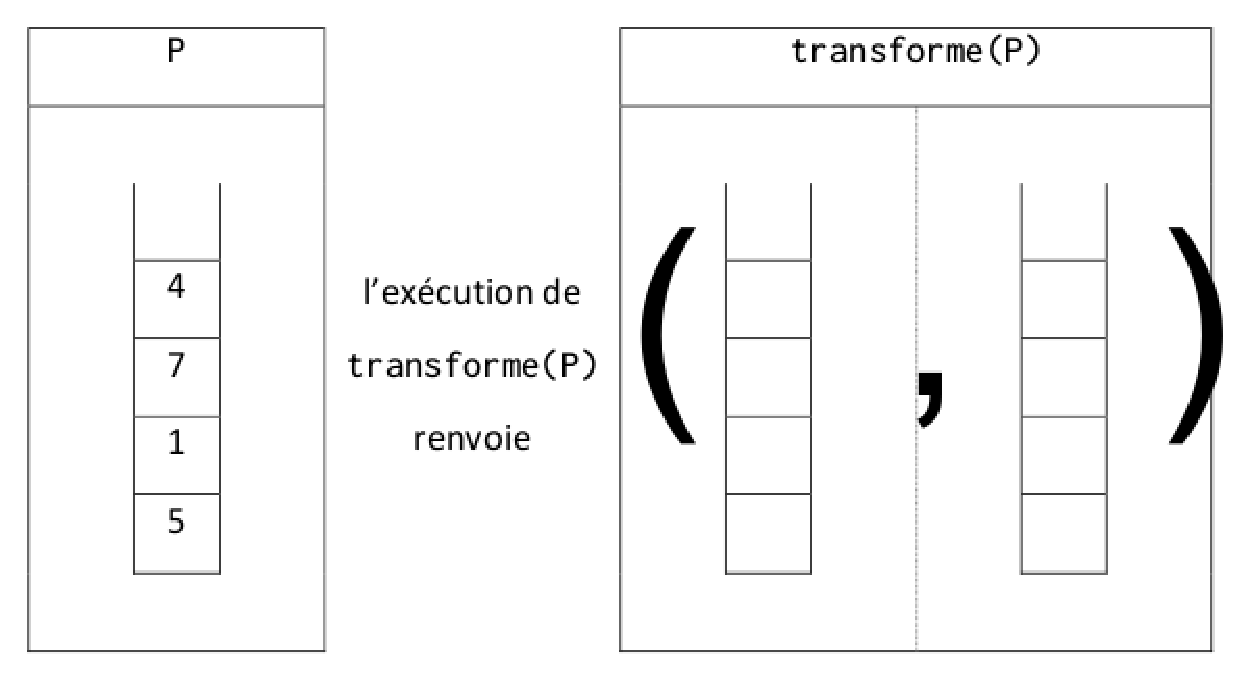
\includegraphics[width=300px]{TypeBac1-a.eps}
\end{center}
\item \textbf{Ecrire} une fonction en langage Python {\tt maximum(P)} recevant une pile {\tt P} comme argument et qui renvoie la valeur maximale de cette pile. On ne s'interdit pas qu'après exécution de la fonction, la pile soit vide.
\FinListe

\vspace{0.2cm}
\large{\bf  Partie B}

On suppose qu'on dispose d'une base de données des processus lancés sur un ordinateur à un instant donné. Cette base de données est constituée d'une seule table appelée {\tt processus} et contenant les champs suivants :
\begin{itemize}
    \item {\tt pid} : le {\sc pid} du processus
    \item {\tt ppid}: le {\sc ppid} du processus
    \item {\tt user}: le nom du propriétaire du processus
    \item {\tt time}: le temps d'exécution du processus (en secondes)
\end{itemize}

\QListe
\item A propos des processus
\SQListe
\item Rappeler rapidement ce qu'est le {\tt pid} d'un processus
\item Parmi les commandes suivantes, indiquer sur votre copie laquelle permet de tuer un processus en cours d'exécution.
    \begin{itemize}
        \item {\tt delete}
        \item {\tt stop}
        \item {\tt remove}
        \item {\tt end}
        \item {\tt kill}
        \item {\tt interrupt}
    \end{itemize}
\item Expliquer pourquoi {\tt pid} peut être utilisé comme clé primaire de cette table et pas {\tt user}
\FinListe
\item Quelques requêtes
\SQListe
\item Ecrire une requête {\sc sql} permettant d'afficher les champs {\tt pid} et {\tt user}.
\item Ecrire une requête {\sc sql} permettant d'afficher les processus de l'utilisateur {\tt root}.
\item Ecrire une requête {\sc sql} permettant d'afficher tous les fils du processus de {\tt pid} 712.
\item Ecrire une requête {\sc sql} permettant d'afficher les {\tt pid} des processus ayant un temps d'exécution supérieur à 50 secondes.
\item Ecrire une requête {\sc sql} permettant d'afficher les processus classés dans l'ordre alphabétique du propriétaire du processus.
\item Ecrire une requête {\sc sql} permettant d'afficher les 5 processus ayant le plus long temps d'exécution.
\FinListe
\FinListe


\end{document}

